\documentclass[10pt]{article}

\usepackage{mathtools}  % need for math tools
\usepackage{amsmath}    % need for subequations
\usepackage{graphicx}   % need for figures
\usepackage{verbatim}   % useful for program listings
\usepackage{color}      % use if color is used in text
\usepackage{subfigure}  % use for side-by-side figures
\usepackage{hyperref}   % use for hypertext links, including those to external documents and URLs


\setlength{\baselineskip}{16.0pt}   
\setlength{\parskip}{3pt plus 2pt}
\setlength{\parindent}{20pt}
\setlength{\oddsidemargin}{0.5cm}
\setlength{\evensidemargin}{0.5cm}
\setlength{\marginparsep}{0.75cm}
\setlength{\marginparwidth}{2.5cm}
\setlength{\marginparpush}{1.0cm}
\setlength{\textwidth}{150mm}

\begin{document}

\begin{center}
{\large Ay190: Computational Astrophysics (Winter Term 2012)} \\
{\large Term Project } \\
{\large Particle–Particle vs. Particle-Mesh for Evaluating Gravitational Forces}\\
\copyright 2012 by Arya Farahi \\
March, 2012
\end{center}

\section{Introduction}

An N-body simulation is a simulation of a dynamical system of particles, usually under the influence of physical forces, such as gravity. In cosmology, they are used to study processes of non-linear structure formation such as the process of forming galaxy filaments, galaxy halos from dark matter in physical cosmology and evolution of dark matter halos, star evolutions, simulation of star clusters, and etc. \\

The main problem in N-body simulation is how to find the gravitational force and then calculating the acceleration of particles in each step time. We used different methods to speed up the computational process. The most simple method is direct gravitational method which in too slow but the most accurate one. In direct gravitational N-body simulations, the equations of motion of a system of N  particles under the influence of their mutual gravitational forces are integrated numerically without any simplifying approximations. Scholars tried to find was to decrease the processing time by doing approximation and applying different tricks to our problem.\\

Another possibility is the particle mesh method. Particle Mesh (PM) is a computational method for determining the forces in a system of particles. These particles could be atoms, stars, or fluid components and so the method is applicable to many fields, including molecular dynamics and astrophysics. The basic principle is that a system of particles is converted into a grid (or "mesh") of density values. The potential is then solved for this density grid, and forces are applied to each particle based on what cell it is in, and where in the cell it lies.\\

Various methods for converting a system of particles into a grid of densities exist. One method is that each particle simply gives its mass to the closest point in the mesh. Another method is the Cloud-in-Cell (CIC) method, where the particles are modelled as constant density cubes, and one particle can contribute mass to several cells.\\

Once the density distribution is found, the potential energy of each point in the mesh can be determined using Fourier transform techniques. Thus it is faster to do a PM calculation than to simply add up all the interactions on a particle due to all other particles for two reasons: firstly, there are usually fewer grid points than particles, so the number of interactions to calculate is smaller, and secondly the grid technique permits the use of Fourier transform techniques to evaluate the potential, and these can be very fast.\\

PM is considered an obsolete method as it does not model close interaction between particles well. It has been supplanted by the Particle-Particle Particle-Mesh method, which uses a straight particle-particle sum between nearby particles in addition to the PM calculation.\\

In this point of view, space is discretised on a mesh and, for the purposes of computing the gravitational potential, particles are assumed to be divided between the nearby vertices of the mesh. Finding the potential energy $\Phi$ is easy, because the Poisson equation\\

\begin{equation}
    \nabla^2\Phi= -\ 4\pi G{\rho},\,
\end{equation}

where $G$ is Newton's constant and $\rho$ is the density (number of particles at the mesh points), is trivial to solve by using the Fourier transform to go to the frequency domain where the Poisson equation has the simple form \\

\begin{equation}
    \hat{\Phi}= -\ 4\pi G\frac{\hat{\rho}}{k^2},
\end{equation}

where $\vec{k}$ is the comoving wavenumber and the hats denote Fourier transforms. The gravitational field can now be found by multiplying by $\vec{k}$ and computing the inverse Fourier transform (or computing the inverse transform and then using some other method). Since this method is limited by the mesh size, in practice a smaller mesh or some other technique (such as combining with a tree or simple particle-particle algorithm) is used to compute the small-scale forces. Sometimes an adaptive mesh is used, in which the mesh cells are much smaller in the denser regions of the simulation.\\

In this project we aim to study the efficiency and accuracy of this method by changing the mesh grid and increasing the number of paricle with compare to the direct gravitational method. In the second part we develope the code for calculating the Fourier transform terms and Inversing the Fourier transform terms into real space. Also because for finding the force between two particles one need to calculate the derivative terms of potential field respect to spacial coordinates. We figure out how to use Fourier transform to calculating the derivating terms. In the third part we apply the developed code for our N-Body problem. And in the forth part we discuss about the results.\\

\section{Fourier transformation}

In this part we develope the computational code for finding the Fourier transformation terms and the method for inversing the Fourier transformation terms into real space. In Fourier transformation is defined:

\begin{equation}
    \hat{f}(k) = \int_{-\infty}^{\infty} f(x)\ e^{- i x k}\,dx,
\end{equation}

for every real number $k$.\\
And the inverse fourier transform defiened:
\begin{equation}
    f(x) = \int_{-\infty}^{\infty} \hat{f}(k)\ e^{ i k x}\,dk,  
\end{equation}
for every real number $x$.\\

There is a good numerical method, Fast Fourier Transform, for calculating these integrals and changing the real space into k space and vice versa, which is coded up in most languages such as MATLAB, Python, C++, FORTRAN, and etc. In this project, FFT used for changing real space into k space. As it was shown, in k-space, forces can be calculating simply by multiplying each component by $k X i$. \\

So first we need to figure out how to work with FFT function in Python, and how to calculate k vector for each component. Based on what is defined in FFT function in Python the k vector is defined with this function for even number of grid cells for each dimention: \\

\begin{verbatim}
def k_space(n,L):
    k = zeros(n)
    if (mod(n,2) == 0):
      for i in range(n/2):
         k[i]     = i * (2*pi/L)
         k[n-1-i] = (-i-1) * (2*pi/L)
      k[n/2]  = 0.0
    return k
\end{verbatim}

Knowing k help us to calculate derivative of out function in k space. So derivative of function is defined:\\

\begin{equation}
    \frac{df(x)}{dx} = \int_{-\infty}^{\infty} i k \hat{f}(k)\ e^{ i k x}\,dk,  
\end{equation}

So the results in k space for each term need to be multiplied by $i k$. For claculating the Force by knowing the potential field one need to get derivative respect to x, y, and z. In our problem, first we calculate the potential field in k space then we find its derivative, and in final step we convert the result in Fourier Space into real space.\\

For checking how FFT works and if it is accurate for claculating the derivative of specific function, an analytical potential function, in this example $f(x,y,z) = x^2 + y^2 + z^2 $, is used to compare the results with the analytical answer. Figure \ref{fig:FourierTest} the red line and blue line, respectivly, is showing the analytical answer and the result of derivative with help of Fourier transformation. And it is possible to show that by increasing the number of cells the relative error would decrease. So it is possible to use this method for finding the 

\begin{figure}[hbt]
  \begin{center}
    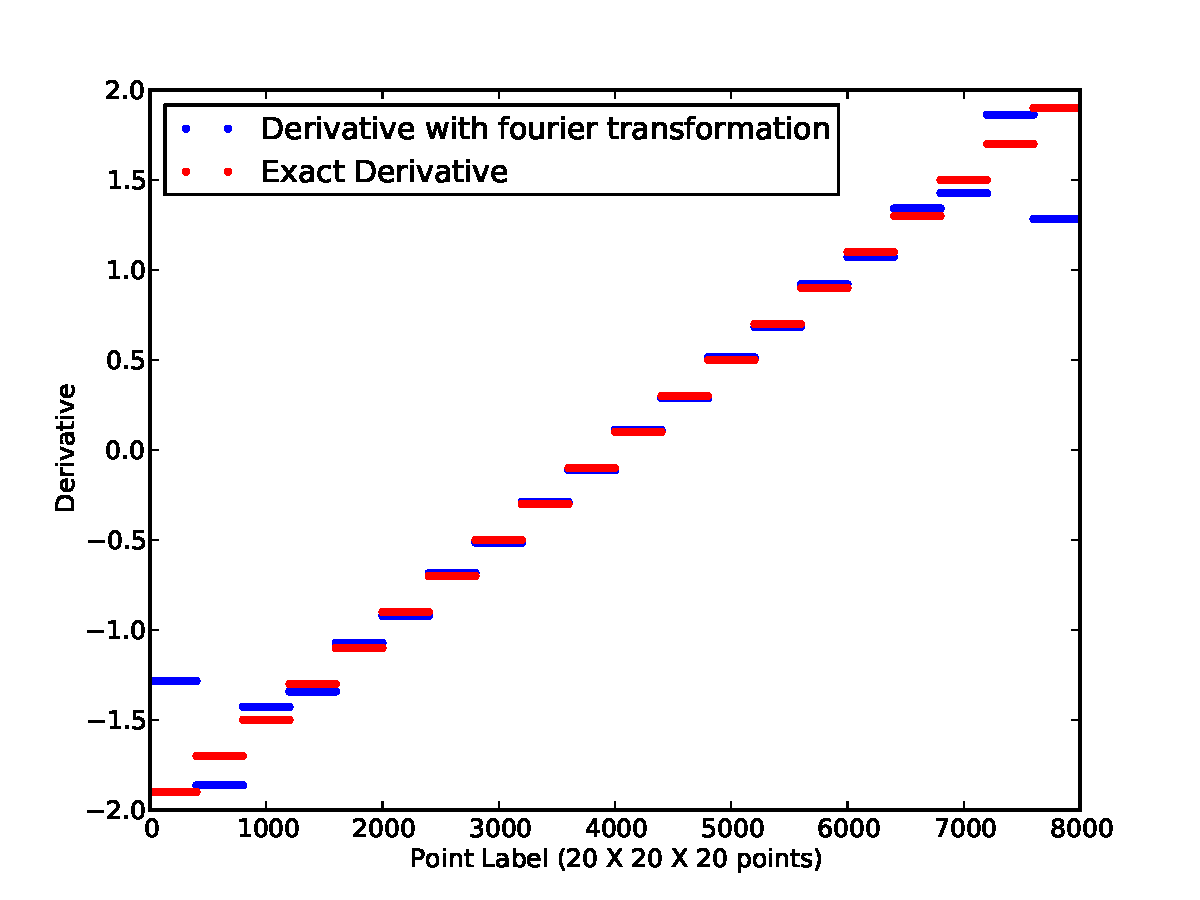
\includegraphics[scale=0.6]{Plots/FourierSeries/plotFourier20.pdf}
    \caption{\label{fig:FourierTest} Plot of derivative of $f(x,y,z) = x^2 + y^2 + z^2$ respect to $x$ for $8000$ point with analytical solution and fourier transformation method.}
  \end{center}
\end{figure}

\section{Developing the computational Code}

In this section, we try to develop the computational code for this problem based on \texttt{FFT} function which is exist in \texttt{Numpy} library in Python. So first of all let's divide our problem into four step. In first step, equation \ref{eq:step1} $\rho$ (density) field in real space is converted to $\rho$ field in k space. In second and third step, equation \ref{eq:step2} and \ref{eq:step3}, $\rho$ field and $\phi$ (potential) field is used for calculating $\phi$ and $F_x$ respectily. And at the final step, $F_x$, which was in k space, is converted into $F_x$ in real space.    

First Step:\\

\begin{equation} \label{eq:step1}
    \hat{\rho}(k) = \int_{-\infty}^{\infty} \int_{-\infty}^{\infty} \int_{-\infty}^{\infty} \rho\ e^{- i \vec{k} . \vec{x}}\,dx^3,
\end{equation}
 
Second Step:\\

\begin{equation} \label{eq:step2}
    \hat{\Phi}_i= - 4\pi G\frac{\hat{\rho}_i}{k^2},
\end{equation}

Third Step:\\

\begin{equation} \label{eq:step3}
    \hat{F}_{ix} = - i k_x \hat{\Phi}_i,
\end{equation}

Fourth Step: \\

\begin{equation} \label{eq:step4}
    F_x = \int_{-\infty}^{\infty} \int_{-\infty}^{\infty} \int_{-\infty}^{\infty} \hat{F_x}\ e^{ i \vec{k} . \vec{x}}\,dx^3,
\end{equation}

First of all, the geometery should divided into numerious grid cells and each grid cell has its own properties, such as density field, potential field, and Force. First for starting to solve the problem we have to think about a way to calculate density field in each cell. For finding the density field there are many methods such as: nearest grid point (NGP), cloud-in-cell (CIC) and triangular-shaped cloud (TSC) methods. In this project we used NGP and CIC for computing the density field in each cell.\\

The following functions calculate the number of particles in each cell which is used to in NGP method, density of each cell based on CIC point of view, and the last one would mesh the geometery (in this problem a cube): \\

\begin{verbatim}
def mass_counter(xmin,xmax,ymin,ymax,zmin,zmax,x,y,z):
    n     = 0
    for i in range(len(x)):
       if ((x[i]>=xmin) and (x[i]<xmax)):
          if((y[i]>=ymin) and (y[i]<ymax)):
             if((z[i]>=zmin) and (z[i]<zmax)):
                n += 1
    return n

def density_CIC(x0,y0,z0,x,y,z,dx):
    mass    = 1.0      # Mass of each particle
    density = 0.0
    for i in range(len(x)):
       if ((abs(x[i] - x0)) < dx and (abs(y[i] - y0) < dx) and (abs(z[i] - z0) < dx) ):
            density += mass*\
                      \((1.0 - abs(x[i] - x0)/dx)*\
                      \(1.0 - abs(y[i] - y0)/dx)*\
                      \(1.0 - abs(z[i] - z0)/dx))
    return density

def mesh_the_volume(xmin,xmax,ymin,ymax,zmin,zmax,x,y,z,n):
    mass     = 1.0      # Mass of each particle
    dx       = (xmax - xmin)/n
    dy       = (ymax - ymin)/n
    dz       = (zmax - zmin)/n
    volume   = dx*dy*dz
    R        = zeros([n,n,n,4])
    l        = 0
    for i in range(n):
      for j in range(n):
        for k in range(n):
          x0min   = xmin + i*dx
          y0min   = ymin + j*dy
          z0min   = zmin + k*dz
          x0max   = xmin + (i+1)*dx
          y0max   = ymin + (j+1)*dy
          z0max   = zmin + (k+1)*dz
          R[i,j,k,1]    = (x0max + x0min)/2.0
          R[i,j,k,2]    = (y0max + y0min)/2.0
          R[i,j,k,3]    = (z0max + z0min)/2.0
#         R[i,j,k,0]    = mass*mass_counter(x0min,x0max,y0min,y0max,z0min,z0max,x,y,z)/volume #NGP
          R[i,j,k,0]    = density_CIC(R[i,j,k,1],R[i,j,k,2],R[i,j,k,3],x,y,z,dx)/volume #CIC
          l += 1
    return R 
\end{verbatim}

Then, after finding density field in each cell, FFT used to convert density field in real space into density field in k space. Also we need a function for calculating k (wavenumber) to compute potential field and then Forces in each direction. We used the following function in our code to calculate the wavenumber based on FFT function, which is just working for 
even numbers of cell: \\

\begin{verbatim}
def k_space(n,L):
    k = zeros(n)
    if (mod(n,2) == 0):
      for i in range(n/2):
         k[i]     = i * (2*pi/L)
         k[n-1-i] = (-i-1) * (2*pi/L)
      k[n/2]  = 0.0
    else:
      print "For odd numbers it is not working ... ! "
      sys.exit()
    return k
\end{verbatim}

Now, simply for calculating each term of the force in k space, each term of density field is multiplied by $i k 4\pi G\frac{\hat{\rho}}{k^2}$. So we have:\\

\begin{equation}
    \vec{\hat{F}}_i = i \vec{k} 4\pi G\frac{\hat{\rho_i}}{k^2},
\end{equation}

The following part of code would do above calculations just for x component of force:

\begin{verbatim}
   density_k = fftn(R[:,:,:,0])
   k_s       = k_space(n,L)
   Fx_k      = zeros([n,n,n],complex)
   for i in range(n):
      for j in range(n):
         for k in range(n):
            k2               = k_s[i]**2 + k_s[j]**2 + k_s[k]**2
            if (k2 != 0.0):
               Fx_k[i,j,k]   = 4.0j*k_s[i]*pi*G*density_k[i,j,k]/k2 
   F = ifftn(Fx_k)
\end{verbatim}

Now simply, by changing the cells number we are able to study the accuracy of this method, compare to direct method, and how increasing the cells would effect on the process time and accuracy. \\

Before going to the next secion it would be good to investigating MP method. It seems that it would not give us good answers. Because first of all we loos informations in each cell and the gravity effect of near particles is not considered with high accuracy. Second we have to convert particles into density field which is kind of approximation and would decrease our accuracy. Third we are not able to compute all temrs of Fourier series so we loos lots of infomation by converting the real space into k space. Fourth, for finding forces for each particle interpolation should be used and it would increase the error. Fifth, but not last, finding the derivative based on Fourier transformation creat some errors so all these thing together would increase the relative error. So it is not expected to find the exact value of forces simply by using this method and not using the other kind of tricks.\\

\section{Results}

In this section we would compare this method with the direct method, which gives us the exact answers. And at the end we would show that just by although it would decrease the computation time, but just by using this method whitout any kind of trick would not give us appropriate answers.\\

\subsection{Mesh study}

In this part we would study the effect of increasing cell numbers on the result of MP method. 50 particles randomly distributed in the cube. Then the each edge of cube divided into 4, 8, 12, and 16 equal part. In means that we have cube with 16, 64, 144, and 256 equal cells. \\

\begin{figure}[htp]
  \centering
  \caption{\label{fig:CompareForce}plot of the value of force in x direction for each particle which is calculated with Mesh particle method and direct method for 16, 64, 144, and 256 cells}
  \begin{tabular}{cc}
    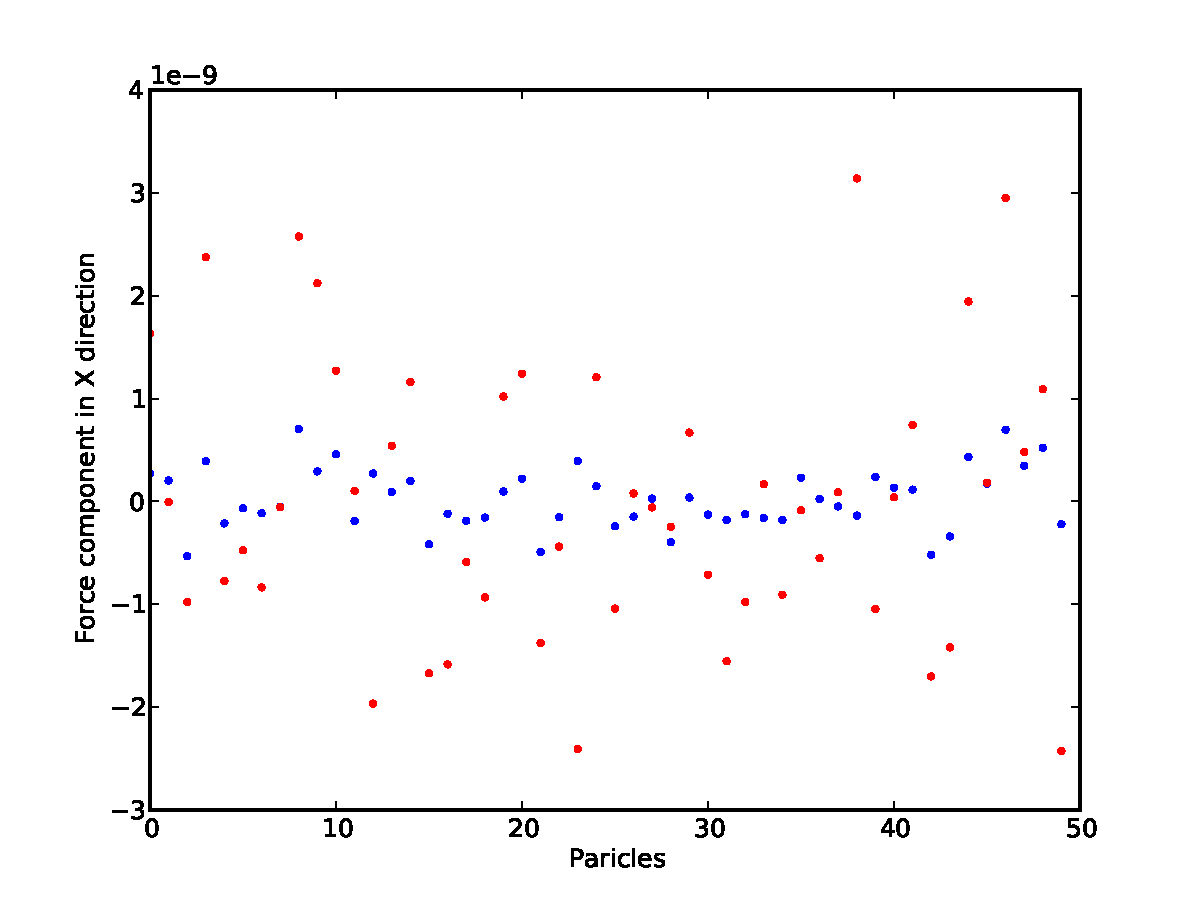
\includegraphics[width=75mm]{Plots/MPCompare/Compare_4.pdf}&
    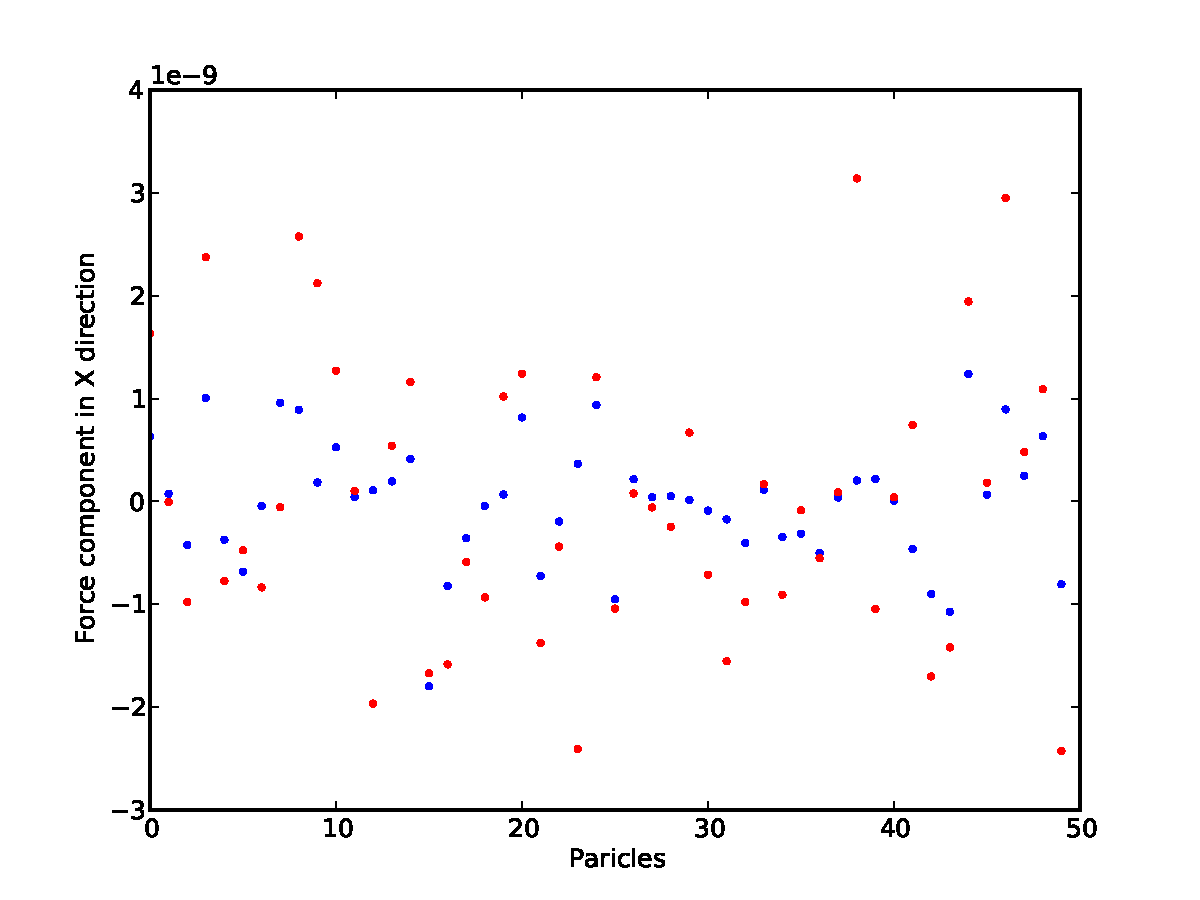
\includegraphics[width=75mm]{Plots/MPCompare/Compare_8.pdf}\\
    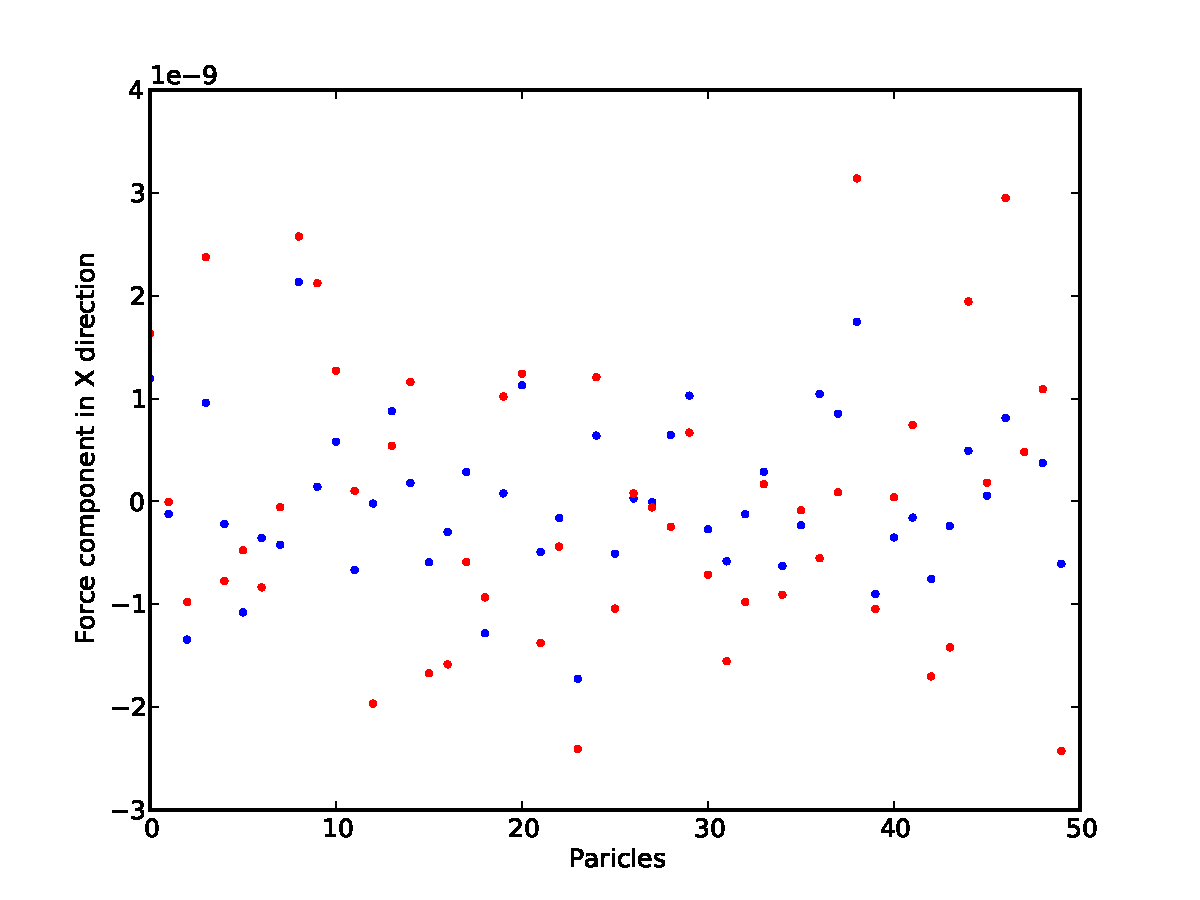
\includegraphics[width=75mm]{Plots/MPCompare/Compare_12.pdf}&
    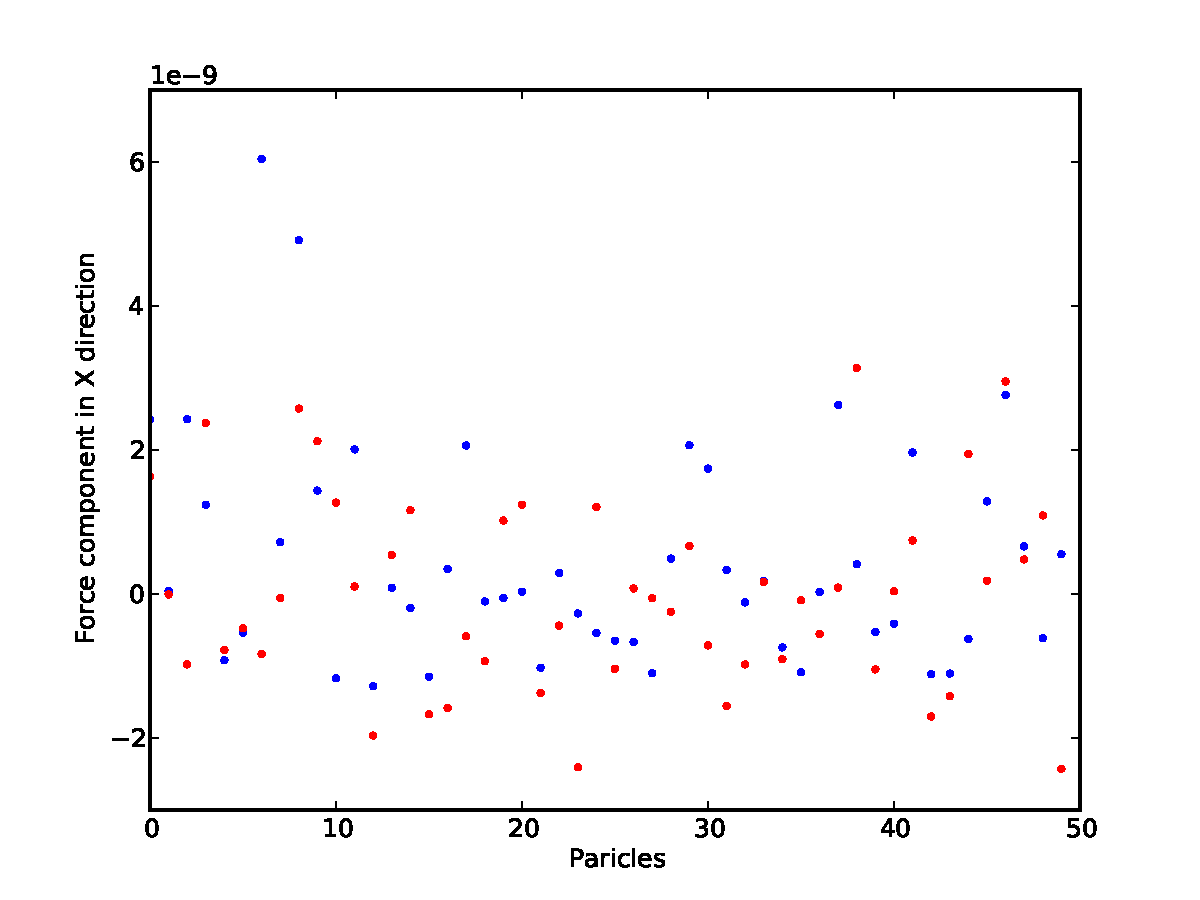
\includegraphics[width=75mm]{Plots/MPCompare/Compare_16.pdf}\\
  \end{tabular}
\end{figure}

\begin{figure}[htp]
  \centering
  \caption{\label{fig:CompareForceErr}Plot of relative error of the value of force in x direction for each particle for mesh particle and direct method for 16, 64, 144, and 256 cells}
  \begin{tabular}{cc}
    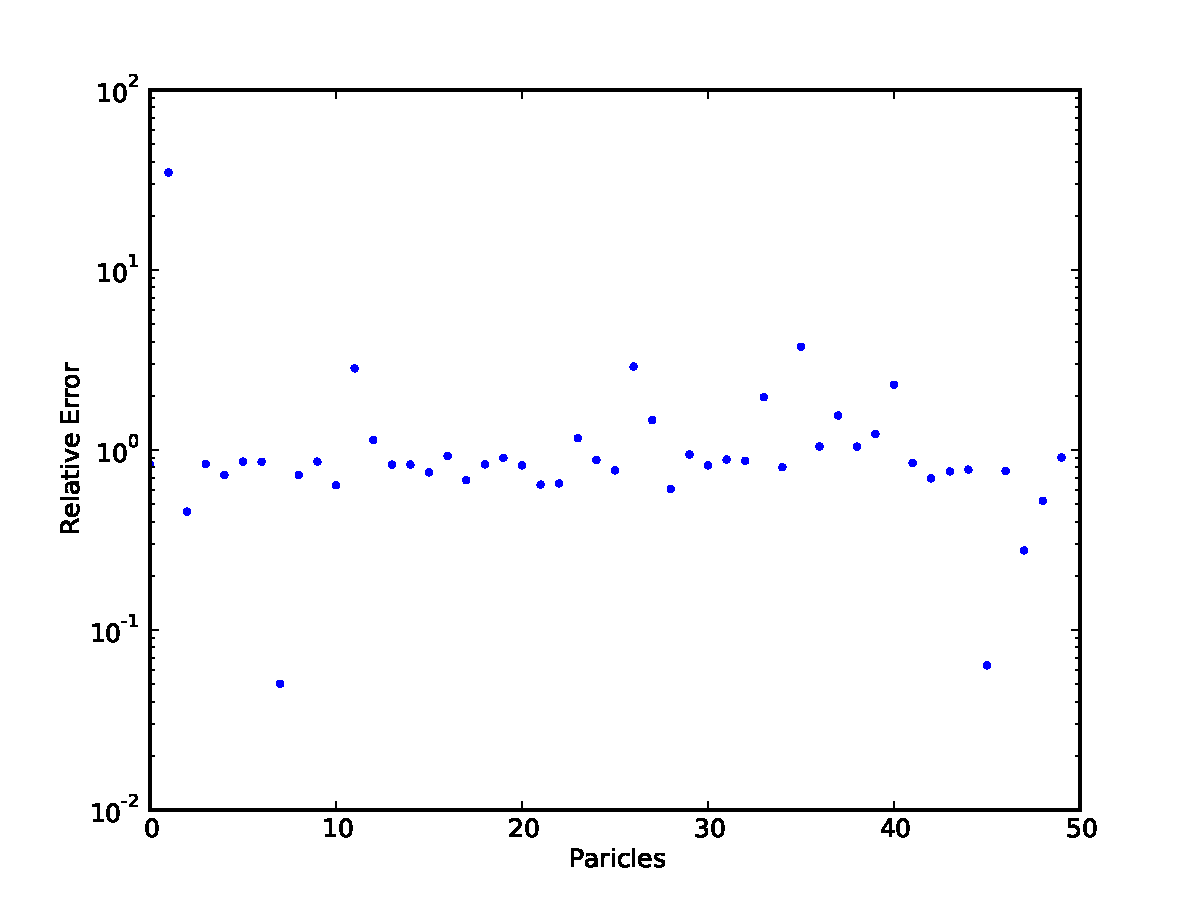
\includegraphics[width=75mm]{Plots/MPCompare/Compare_4_error.pdf}&
    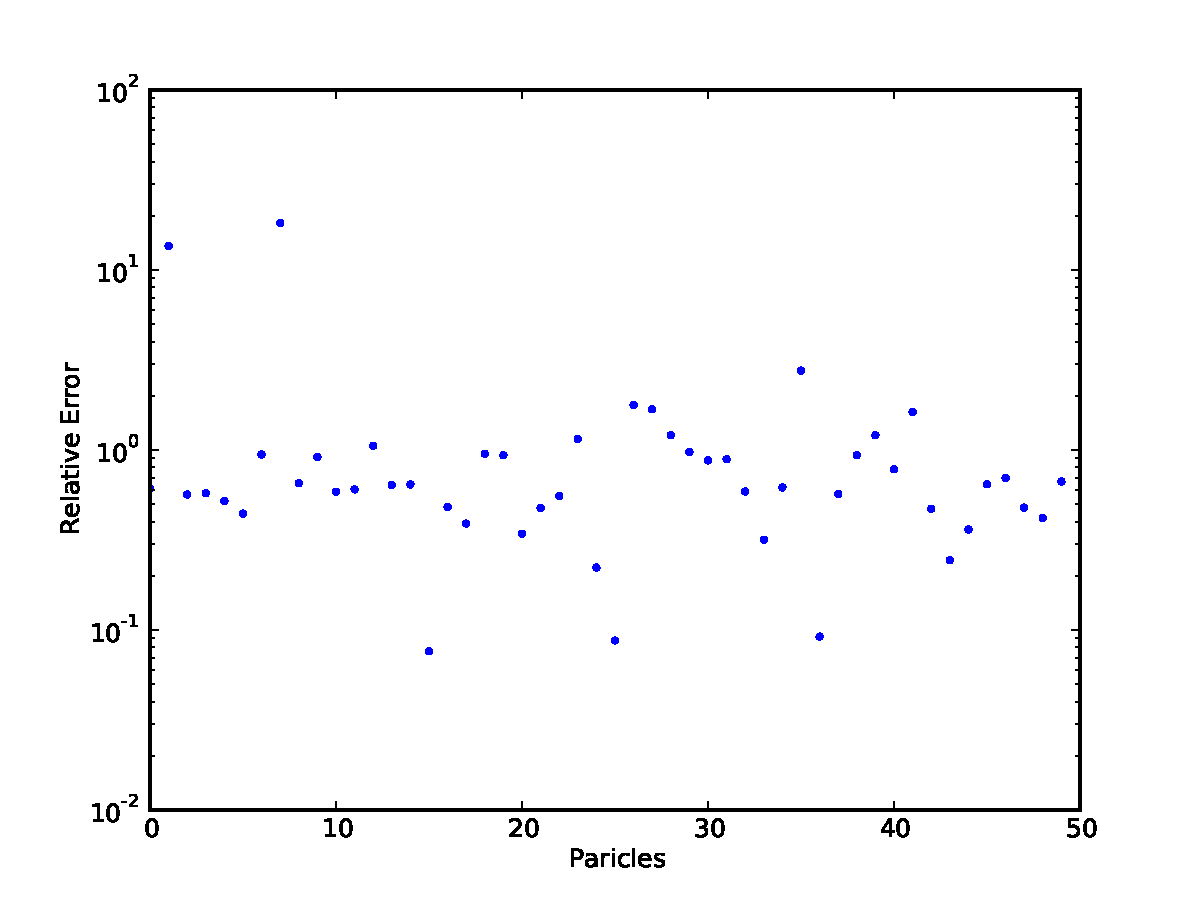
\includegraphics[width=75mm]{Plots/MPCompare/Compare_8_error.pdf}\\
    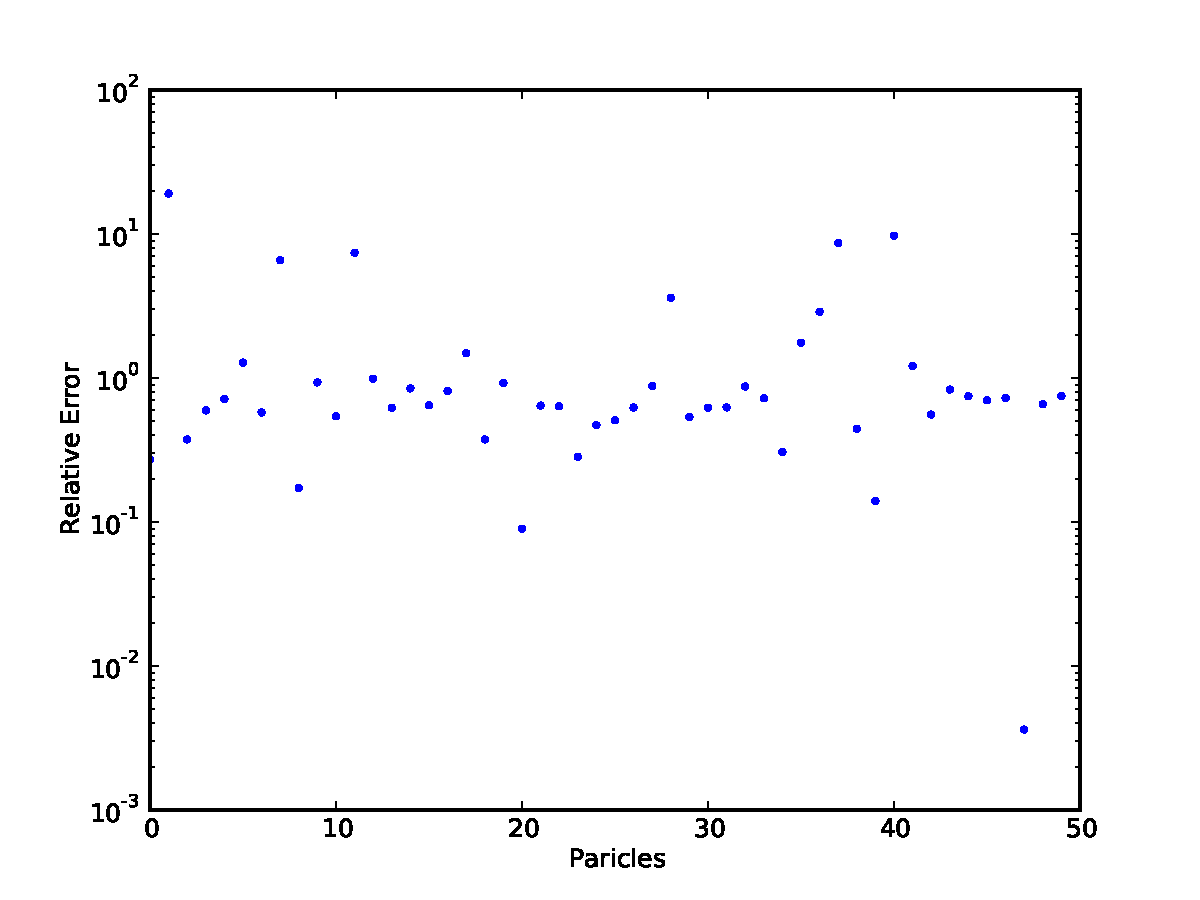
\includegraphics[width=75mm]{Plots/MPCompare/Compare_12_error.pdf}&
    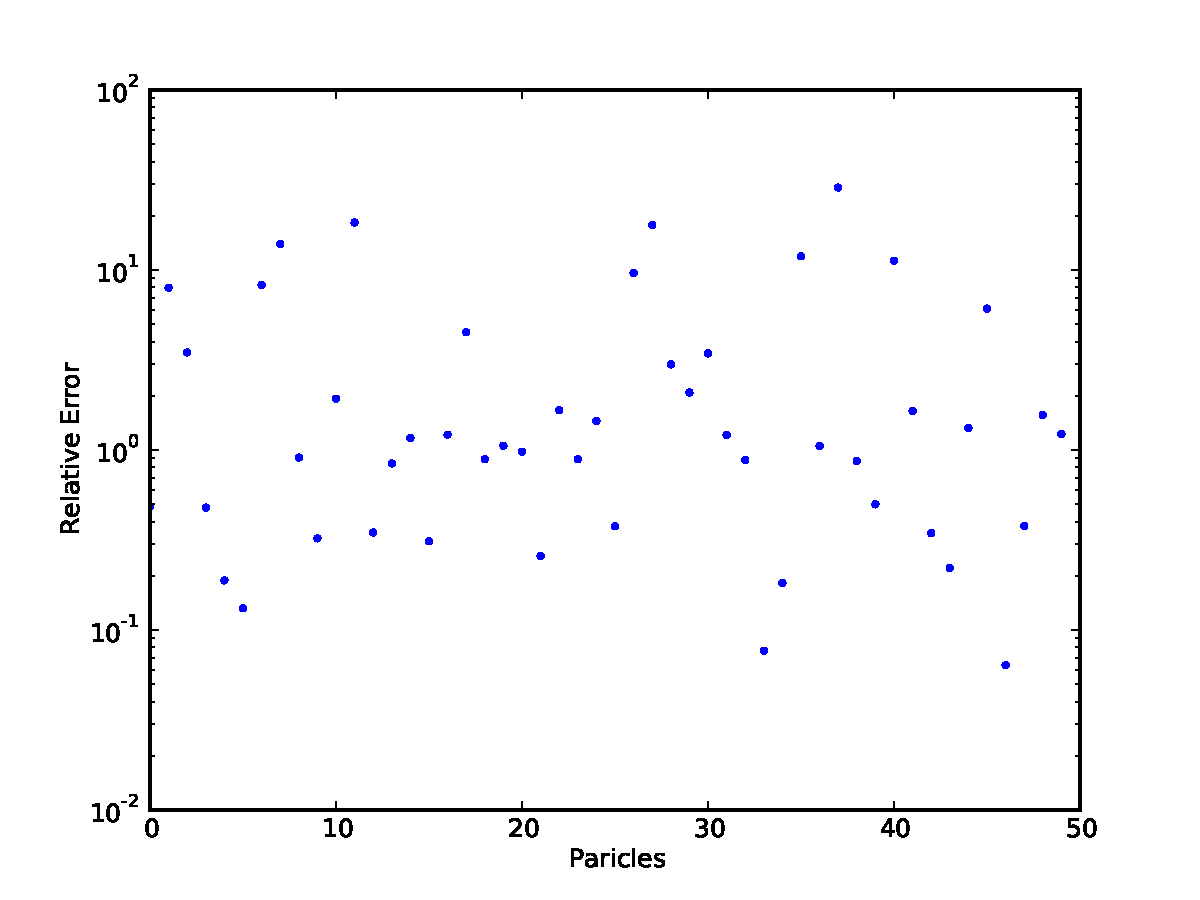
\includegraphics[width=75mm]{Plots/MPCompare/Compare_16_error.pdf}\\
  \end{tabular}
\end{figure}

Figure \ref{fig:CompareForce} shows the value of force in x direction for each particle which is calculated with Mesh particle method and direct method for 16, 64, 144, and 256 cells and figure \ref{fig:CompareForceErr} shows the relative error of the value of force in x direction for each particle for mesh particle and direct method 16, 64, 144, and 256 cells. Based on these plots it seems that the error is decreasing as the number of cells is increasing. But though the error is decreasing but variance is increasing so the force is not accurate for number of particles. So if we aim to calculate force for each particle more accuratly we nned to combine mesh particle method with direct method. It means that for near particles direct method should be used for calculating the force and for distant particles mesh particle method is a good approximation. Anyway, Mesh particle method is not an accurate method for finding the exact force of each particle but as whole the relative error is decreasing with increasing the number of cells. 

\subsection{Time study}

\begin{figure}[hbt]
  \begin{center}
    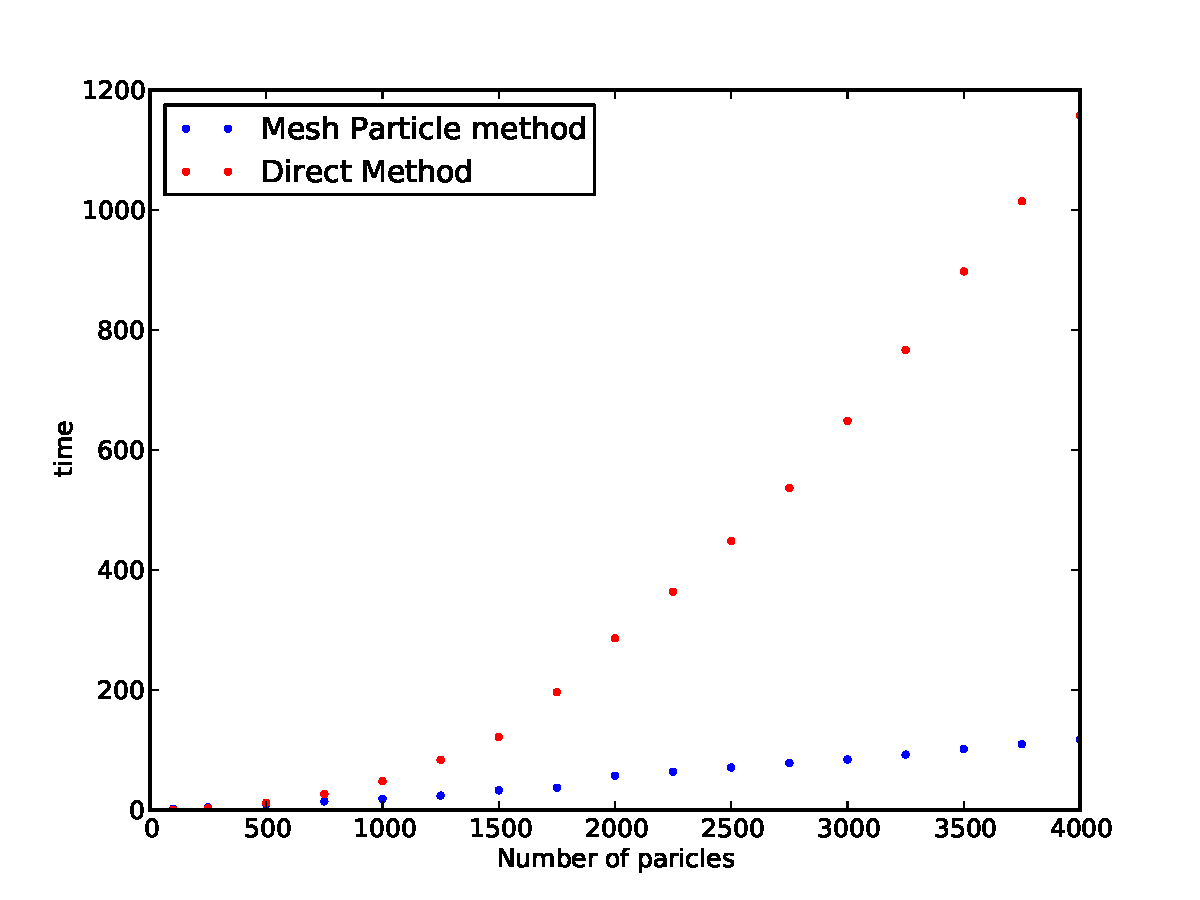
\includegraphics[scale=0.6]{Plots/time/timeI.pdf}
    \caption{\label{fig:TimeI} The plot is showing how duration of time of solution is changing by number of particles.}
  \end{center}
\end{figure}

\begin{figure}[hbt]
  \begin{center}
    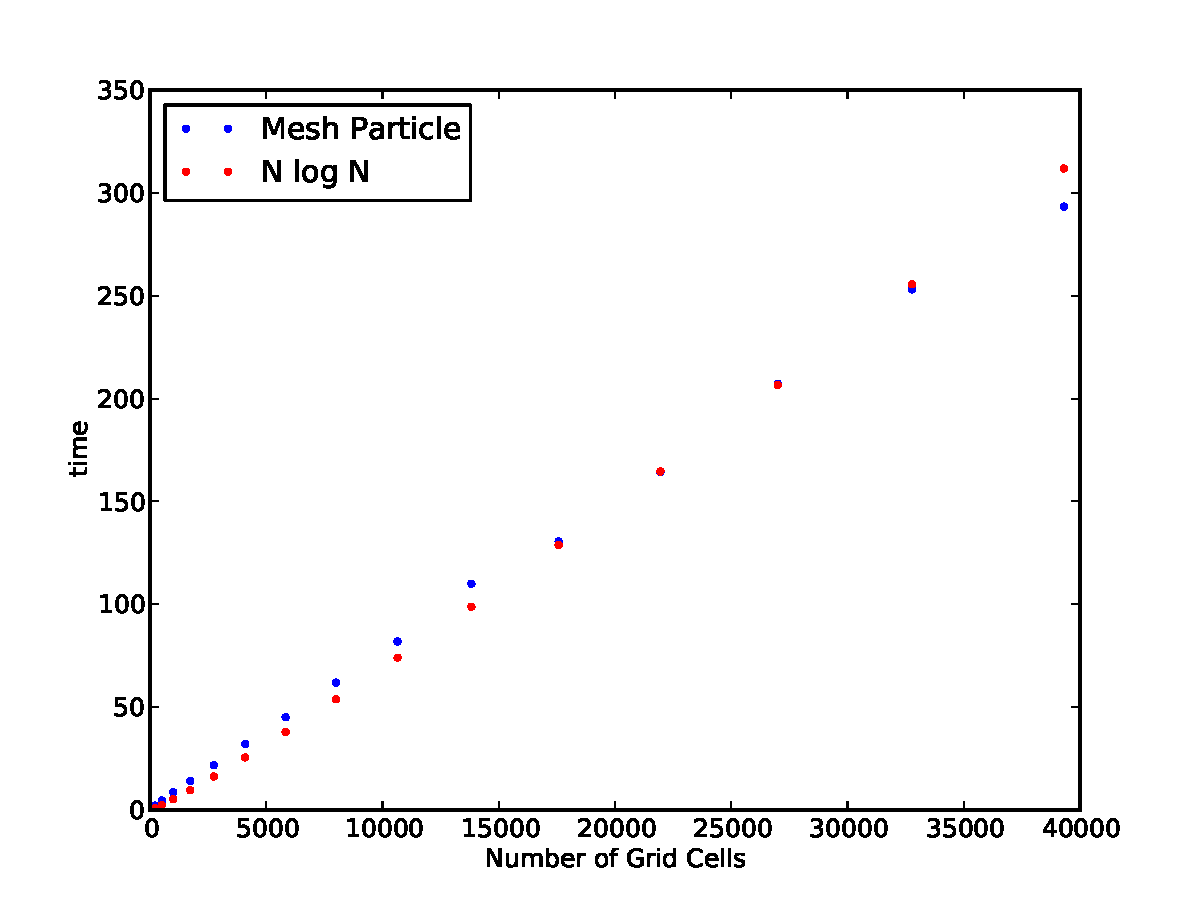
\includegraphics[scale=0.6]{Plots/time/timeII.pdf}
    \caption{\label{fig:TimeII} The plot is showing how duration of time of solution is changing by number of grid cells for fixed number of particles.}
  \end{center}
\end{figure}

It is expected that the order of particle mesh algorithms is $\mathcal{O}(N + N_g \log N_g)$ and the order of direct method is $\mathcal{O} (N^2)$. In this section we want to study the order of our algoritms. Figure \ref{fig:TimeI} shows that mesh particle method's dependence to the number of particle, as we expected, is linearly changing and direct method's order is $N^2$. Also, figure \ref{fig:TimeII} shows that the order of the problem with changing the number of grid cells is acting like $N_g \log N_g$.

\subsection{Conclusion}

There are many ways to spped up the computational process. It is a good idea to use particle mesh method but it is not enough. Because it can not predect the forces for each particl with high accuracy, specially forces between neighbour particles. prticle mesh method is considered an obsolete method as it does not model close interaction between particles well. It has been supplanted by the Particle-Particle Particle-Mesh method, which uses a straight particle-particle sum between nearby particles in addition to the PM calculation. But by increasing the number of grid cells the error would decreas and the order of particle mesh method, with fixed number of cells, is linear. So this method help us to speed up the computational process, and one need to combine this method with another method, like particle particle method, to increase the accuracy.\\

\section{Note}
There are number of codes which one of them is calculating force with direct method, the other one uses mesh to compute the forces, and the last one is OCT tree method which is complteley different from the others. Also in the process of developing codes I have coded up 3 dimentional Fourier Series module which compute number of terms for Fourier Series and convert Fourier Series into real space, which is not used in this project because in this project we have to use Fourier trasformation which is completely different from Fourier Series. But for periodec problems one can use Fourier Series.

\pagebreak

\end{document}
